\chapter {Introduction}

\section {Estimation of MIMO channel}

Multiple-input multiple-output (MIMO) communication system will be part of the 5G specification \cite {RSM13}.
With a large number of antennae on both transmitter and receiver ends, MIMO is expected to provide a large signal gain.
The appeal of MIMO includes multiplexing gain (parallel transmission of data), diversity gain (redundant transmission with space-time coding), and antenna gain (suitable beamforming to improve the signal level).
Besides, the millimeter wave (mm-wave) is suggested, since its smaller wavelength (and thus higher frequency) makes wider bands available.
Moreover the antennae may be closer-spaced, allowing us to increase their number.

However, MIMO also gives rise to higher complexity, hence higher hardware overhead and power consumption.
To obtain channel state information (so that channel capacity can be known for instance), new algorithms have to address these issues.
Not only is the channel estimation difficult, due to a large antennae array, but the transmission in higher frequency is subject to noise corruption too.
As a result, conventional training-based algorithms lead to considerable time and space complexity.



\section {Compressive sensing}

If we consider a slow varying MIMO channel for simplicity, in terms of a channel representation, to estimate the channel is to determine the parameters of the representation.
We shall see it amounts to invert a linear system whose dimension is the number of antennae, which is not very effective.
Fortunately, physical evidence has suggested that mm-wave channel are poor in scattering \cite {ALS14}, which reduces the number of paths, and it is now that a recent development called compressive sensing may help.

\bigskip
\begin {figure} [hbt]
\centering
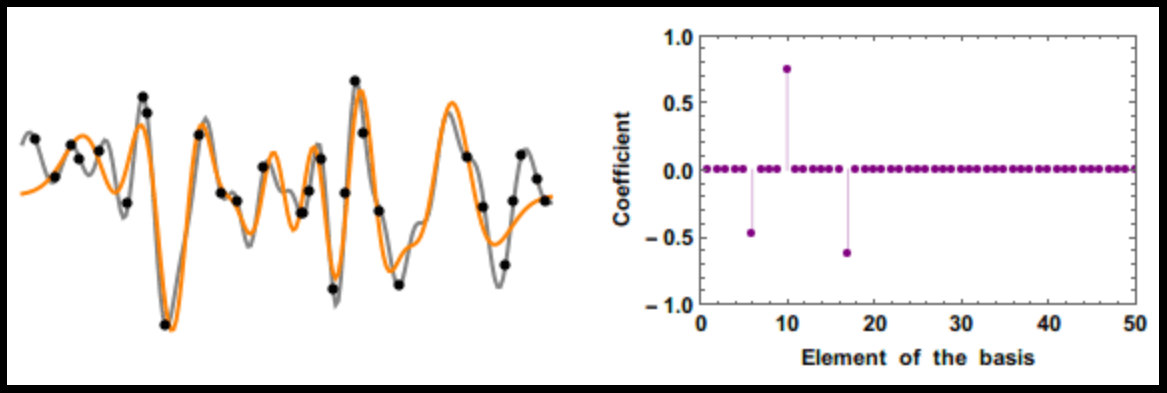
\includegraphics [width = \textwidth] {compressive-sensing.png}
\caption {
A conceptual illustration of compressive sensing.
(Retrieved from \href {commons.wikimedia.org/wiki/File:Orthogonal_Matching_Pursuit.gif} {Wikimedia Commons})
}
\end {figure}
\bigskip

Figure 1 shows a generic situation in which a signal is crowded in the given basis, but is sparse in transformed basis.
The black line on the left is the original signal, and the yellow line is the reconstruct signal.
If the signal is sparse on certain new basis, as shown in the right, then for a good approximation, we may take only the largest components for reconstruction.

Generally speaking, compressive sensing aims to reconstruct a underdetermined linear system, when the sparsity of solution guarantees successful recovery for most cases.
More measurements are required to recover the signal in the nonsparse basis, while fewer suffice in the sparse basis.
But, even if we are sure that the sparse basis exists, its construction is another undertaking.

Let us say the number of model parameters \m {N_p \in \mathbb {N}} is much larger than the number of measurements \m {N_m \in \mathbb {N}}, that is,
%
\DispNum {N:p:Nm:Nm} {
N_p \gg N_m \\
}
%
To start, consider \m {\V {x}, \V {x}' \in \mathbb {K} ^{N_p}} and \m {\M {Q} \in \mathbb {K} ^{N_m \D  N_p}}, and the linear system
%
\DispNum {y:y:Qx:Qx} {
\V {y}
=\M {Q} \V {x} \\
}
Certainly, if \m {\M {Q} \RB {\V {x}_1 - \V {x}_2} = 0}, then \m {\V {x}_1, \V {x}_2} are indistinguishable.
But if \m {\V {x}} is sparse, can we rule out some of the possibilities?

To be precise, we say \m {\V {x}} is \m {s}-sparse, if only at most \m {s} components of \m {x} is nonzero.
That is, if there is some \m {\mathcal {A} \subseteq \CB {0, \dots, N_p-1}} such that
%
\DispNum {x:A:x::x:} {
\V {x} _{\SB {\mathcal {A}}}
=\V {x} \\
}
%
with
%
\DispNum {A:A:s::s:} {
\Nm {\mathcal {A}} \leq s. \\
}

Candès and Tao \cite {Can05}, one of the earlier investigations on compressive sensing, showed that, in the noiseless case, a \m {\ell_1}-minimization program recovers the \m {N_m}-dimensional signal, with \m {N_p} measurements, under overwhelming probability.

As an application, it often occurs that a camera takes a high definition photo, and compresses the image later.
But it may be desirable that a camera equipped with fewer sensors shall take a lower resolution photo to save storage, and shall recover the image later.
Such advantage can be useful in medical imaging, since it is not only expensive, but also harmful, to take too many images, while the accuracy is critical to the diagnosis too \cite {CaT07}.



\section {The Dantzig Selector}

If the linear system is moreover subject to noise \m {z},
%
\DispNum {y:y:Qx:xz} {
\V {y}
=\M {Q} \V {x} + \V {z} \\
}
is it still possible to recover \m {\V {x}}?

We introduce some conventions.
For \m {\mathcal {A} \subseteq \CB {0, \dots, N_p-1}}, denote
%
\Disp {
\V {x}  _{\SB {\mathcal {A}}}
=\sum _{i \in \mathcal {A}} \V {v} \V {u} _{i} \\
%
\M {Q}  _{\SB {\mathcal {A}}}
=\sum _{i \in \mathcal {A}} \M {Q} _{\SB {:,i}} \\
}
%
That is, respectively, the components of \m {\V {x}}, and the columns of \m {\M {A}}, that have indices in \m {\mathcal {A}}.


\Result
{Definition}
{
For fixed \m {s =0, \dots N_p -1}, we say that \m {\M {Q}} satisfies \m {\d_s}-restricted isometry property (hereafter \m {\d_s} RIP) of sparsity \m {s} with respect to \m {0 \leq \d_s \leq 1}, if for all \m {s}-sparse \m {\V {x}}
%
\DispNum {1:2:Qx:22} {
\RB {1-\d_s} \VNm {\V {x}} _2 ^2
\leq \VNm {\M {Q} \V {x}} _2 ^2 \\
%
\leq \RB {1+\d_s} \VNm {\V {x}} _2 ^2 \\
}
}
%
It helps to think that \m {\M {Q}} is almost unitary up to relative error \m {\d_s}.

For concreteness, say \m {\V {z}} is an i.i.d.\ normalized random normal vector.
If so, a stronger result was established \cite {CaT07} that, with another \m {\ell_1} minimization program called Dantzig selector (hereafter DS), recovery under the noisy case is again possible under high probability.

\Result
{Algorithm}
{
\begin {itemize}
\item Input \m {\M {Q} \in \mathbb {R} ^{N_m \D N_p}} and \m {\V {y} \in \mathbb {R} ^{N_m}}.
%
\item Compute the convex program
%
\DispNum {h:h:mi:yg'} {
\hat {\V {h}}
\leftarrow \begin {cases}
\Min {\V {h}'} & \VNm {\V {h}'} _1 \\
%
\mathrm {subject} \; \mathrm {to} \quad & \VNm {\M {Q}^\dagger \RB {\M {Q} \V {h}' -\V {y}}} _\infty \leq \g \\
\end {cases} \\
}
\item Output \m {\hat {\V {h}}}.
\end {itemize}
}

Algorithm [2] recovers \m {\V {x}} with the expected error norm bounded with overwhelming probability.
The \m {\ell_1}-minimization problem with \m {\ell_\infty}-constraint may be recast as a linear Program, rendering convex programming technique applicable.
This allows techniques from convex optimization to be used, and Candès and Romberg provided an implementation on their website \cite {CaR05}.

Here the constant \m {\d_s} in Definition [1] is significant, since we can't just take \m {\M {Q}} to be any unitary matrix, for which \m {\d_s =0}.
A common approach is choosing i.i.d.\ entries of \m {\M {Q}}, and it was established by Baraniuk et.\ al.\ \cite {BDD08} that if \m {\VNm {\M {Q} \V {x}}} concentrates sharply, \m {\M {Q}} has RIP for overwhelming probability, but it remains to conceive an algorithm that efficiently generates RIP matrices.

Back at the ranch, recall that the channel estimation has been considered infeasible in the MIMO setting, but luckily, physical evidences suggest that mm-wave channels are sparse in the number of paths.
An early attempt to apply compressive sensing was Bajwa et.\ al.\ \cite {BHS10}, where they argued that if the \m {\ell_0}-norm of the channel matrix may be bounded by a constant, DS may be applied to estimate the time-dependent single-antenna channel response.
The accompanying note by the same researchers \cite {BHR08} showed that \m {X} has RIP for overwhelming probability, justifying their work.



\section {Orthogonal Matching Pursuit}

At the same time, Tropp and Gilbert \cite {TrG07b} suggested likewise that a greedy algorithm called orthogonal matching pursuit (OMP) which also aims to reconstruct a sparse signal in an underdetermined system.
Again consider the situation of \ref {y:y:Qx:xz}.

\Result
{Algorithm}
{
\begin {itemize}
%
\item Input \m {\M {Q} \in \mathbb {R} ^{N_m \D N_p}} and \m {\V {y} \in \mathbb {R} ^{N_m}}, \m {\eta >0}.
%
\item Initialize
%
\Disp {
\V {r}
\leftarrow \V {y} \\
%
S
\leftarrow \varnothing \\
}
%
\item Start the loop with counter \m {i \leftarrow 1}.
%
\item Find
%
\DispNum {n:n:n0:nr} {
n
\leftarrow \underset {n' =0, \dots, N_p-1} {\mathrm {argmax}}
\Nm {\M {Q} _{\SB {:,n'}} \V {r}} \\
}
%
and append \m {S \leftarrow S \cup {n}}.
%
\item Compute
%
\DispNum {Q:Q:QS:Qy} {
\M {Q} ^\ddagger
\leftarrow \RB {\M {Q} _{\SB {S}} ^\dagger \M {Q} _{\SB {S}}} ^{-1} \M {Q} _{\SB {S}} ^\dagger \\
%
\V {r}
\leftarrow \V {y} -\M {Q} _{\SB {S}} ^\dagger \M {Q} ^\ddagger \V {y} \\
}
%
\item Break if
%
\DispNum {r:2:h':h'} {
\VNm {\V {r}} _2
<\eta \\
}
%
otherwise, go to step 4.
%
\item Output 
%
\DispNum {g:g:Qy:Qy} {
\hat {\V {g}}
\leftarrow \M {Q} ^\ddagger \V {y} \\
}
\end {itemize}
}
%
The columns of \m {\M {Q}} are chosen greedily, and we expect its columns to span \m {\V {x}}, playing a role similar to the sensing matrix in the case of DS.
In each step, we estimate the noise \m {\V {r}}, and find a new column most correlated with it, to refine the estimation for \m {\V {x}}.
From Tropp and Gilbert \cite {TrG07a}, the probability that OMP recovers \m {\V {x}} completely is overwhelming.

OMP has since been pervasively used for channel sensing.
Alkhateeb et.\ al.\ \cite {AEL14} proposed an adaptive algorithm with a beam codebook for quantized angles.
Alkhateeb, Leus, and Heath Jr.\ \cite {ALH15} examined the trade-off between number of measurement and accuracy for an all-phase-shifter beamformers based on nonuniform fixed set of angles.
Gao et.\ al.\ \cite {LGC16} proposed a jointly reconstruction, with a modified OMP, of several high-dimensional sparse signals.
Hu, Wang, and He \cite {HWH13} applied OMP to estimate quantized path delay of OFDM subcarriers of stationary channel gain.
Lee, Gil, and Lee \cite {LGL16} considered a hybrid system, where the effective beamformer serves as sensing matrix, based on a designed set of angles.
Manoj and Kannu \cite {MaK17} studied the sparse condition on submatrices of the signal for successful reconstruction.
Gurbuz, Yapici, and Guvenc \cite {GYG18} introduced perturbation on the angles which the sensing matrix based on.
Panayirci et.\ al.\ \cite {PAU19} proposed a concatenation of max-likelihood estimation of model parameters, and maximum-a-posteriori estimation of channel gains, by virtue of OMP.

Performance guarantee of OMP is also studied on various conditions.
Cai, Wang, and Xu \cite {CWX10}, gave a new bound on performance of OMP under assumption of low coherence of columns of matrices, instead of almost unitarity.
Cai and Wang \cite {CaW11} extended the study to DS and other convex programs for sparse recovery, and Ben-Haim et.\ al.\ \cite {BEE10} followed up and refined their bounds, concluding that OMP is better for low SNR scenario, and DS is better for high SNR.



\section {Contribution}

The literature on channel estimation favors OMP for its low complexity, but we wonder how greedy algorithms, such as OMP, compare to convex programs, such as DS.
It might be that greedy algorithms trade precision for complexity, and that the opposite is true of convex programs.

In this treatise, we consider a hybrid system with uniform linear array as in Lee, Gil, and Lee \cite {LGL16}.
They proposed a beamformer shown to be optimal, jointly designed on both ends by a nonconvex optimization program, and due to its difficulty they have made considerable approximation.
Is the approximated design still optimal, or are the angles of sensing matrix not sufficiently precise?

In chapter 2 we shall see that our proposed effective beamformer has RIP for high probability, which may serve as the sensing matrix for DS.
In chapter 3, along the lines of Candès and Tao \cite {CaT07}, we give a quantitative bound (which holds for high probability) on expected error norm.
In chapter 4, we remark that DS can be cast as a linear program, for which more efficient algorithms exist.
Numerical results show that in our problem configuration, DS is superior to other methods.
Indeed, DS is much more accurate than the least square, and both OMP and Lasso often fails.






